\documentclass[11pt,a4paper]{article}

% Pacchetti
\usepackage[utf8]{inputenc}
\usepackage[T1]{fontenc}
\usepackage[italian]{babel}
\usepackage{geometry}
\geometry{a4paper, margin=2.5cm}
\usepackage{amsmath, amssymb}
\usepackage{graphicx}
\usepackage{booktabs}
\usepackage{caption}
\usepackage{float}
\usepackage{array}
\usepackage{xcolor}
\usepackage[hidelinks]{hyperref}
\usepackage{enumitem}

\title{DataMedical Cost Personal Datasets}
\author{Cristian Trofusha, Samuele Epiceno, Giuseppe Antonio Arcuri, Miriam Formaro}
\date{\today}

\begin{document}

\maketitle
\tableofcontents
\newpage

% =======================================================================
\section{Introduzione}
% =======================================================================

\subsection{Descrizione del dataset}
Il dataset \emph{Medical Cost Personal Datasets} raccoglie $n=1338$ osservazioni
relative a beneficiari di polizze assicurative sanitarie negli Stati Uniti.
Per ciascun individuo sono disponibili $7$ variabili:

\begin{itemize}[nosep]
    \item \textbf{charges} (variabile target, continua): spesa medica annua
    addebitata dall'assicurazione, in USD;
    \item \textbf{age} (continua): età dell'assicurato, da 18 a 64 anni;
    \item \textbf{sex} (categorica): \texttt{male} / \texttt{female};
    \item \textbf{bmi} (continua): indice di massa corporea ($\mathrm{kg/m^2}$);
    \item \textbf{children} (discreta): numero di figli a carico coperti dalla polizza, da 0 a 5;
    \item \textbf{smoker} (categorica): \texttt{yes} / \texttt{no};
    \item \textbf{region} (categorica): area residenziale USA (\texttt{northeast},
    \texttt{northwest}, \texttt{southeast}, \texttt{southwest}).
\end{itemize}

Dopo la rimozione di un'osservazione duplicata (identica su tutte le variabili),
il dataset di lavoro consta di $n=1337$ osservazioni, senza valori mancanti.

\subsection{Obiettivi dell'analisi}
L'analisi persegue tre obiettivi complementari:
\begin{enumerate}[nosep]
    \item \textbf{Descrittivo}: visualizzare la distribuzione di \texttt{charges}
    e le relazioni con i regressori disponibili;
    \item \textbf{Inferenziale}: stimare un modello di regressione lineare che
    identifichi i regressori statisticamente significativi della spesa
    sanitaria, valutandone la forma funzionale ottimale, la significatività
    congiunta e individuale dei regressori, e gestire l'eventuale presenza di multicollinearità
    ed eteroschedasticità;
    \item \textbf{Predittivo}: confrontare tecniche di regolarizzazione
    (Ridge, LASSO, Elastic Net) con l'OLS classico in termini di errore di
    previsione fuori campione, valutandone la capacità di selezione automatica
    delle variabili.
\end{enumerate}

\subsection{Risultati attesi}
Sulla base della letteratura relativa a questo dataset e dell'evidenza
grafica preliminare, ci si attende che lo stato di fumatore (\texttt{smoker})
sia il principale determinante della spesa, seguito da età e BMI, con un
effetto marginale del numero di figli; le variabili \texttt{sex} e
\texttt{region} sono attese come non (o debolmente) significative.

% =======================================================================
\section{Descrizione del dataset e Analisi Preliminare}
% =======================================================================

\subsection{Statistiche descrittive}
La Tabella~\ref{tab:descrittive} riporta le statistiche descrittive delle
variabili numeriche.

\begin{table}[H]
\centering
\caption{Statistiche descrittive delle variabili numeriche ($n=1337$)}
\label{tab:descrittive}
\begin{tabular}{lrrrrrr}
\toprule
Variabile & Media & Std & Min & Q1 & Mediana & Max \\
\midrule
age      & 39.22 & 14.04 & 18.00 & 27.00 & 39.00 & 64.00 \\
bmi      & 30.66 & 6.10  & 15.96 & 26.29 & 30.40 & 53.13 \\
children & 1.10  & 1.21  & 0.00  & 0.00  & 1.00  & 5.00 \\
charges  & 13\,279.12 & 12\,110.36 & 1\,121.87 & 4\,746.34 & 9\,386.16 & 63\,770.43 \\
\bottomrule
\end{tabular}
\end{table}

Le variabili categoriche mostrano le seguenti frequenze: \texttt{sex}
sostanzialmente bilanciato (50.5\% \emph{male}, 49.5\% \emph{female});
\texttt{smoker} fortemente sbilanciato (79.5\% \emph{no}, 20.5\% \emph{yes},
coerente con la prevalenza reale del fumo); \texttt{region}
pressoché equidistribuita (southeast 27.2\%, le altre tre $\approx$24\%
ciascuna).

\subsection{Codifica delle variabili categoriche}
Le variabili categoriche sono state trasformate in variabili dummy (0/1)
mediante \emph{one-hot encoding}, escludendo la prima categoria in ordine
alfabetico per ciascuna variabile al fine di
evitare la trappola delle \emph{dummy}, ossia la collinearità perfetta che si
avrebbe includendo tutte le categorie insieme all'intercetta:
Le categorie di riferimento (corrispondenti a coefficiente nullo
per costruzione) sono: \texttt{sex}=\emph{female}, \texttt{smoker}=\emph{no},
\texttt{region}=\emph{northeast}. Si ottengono così 8 regressori:
\texttt{age}, \texttt{bmi}, \texttt{children}, \texttt{sex\_male},
\texttt{smoker\_yes}, \texttt{region\_northwest}, \texttt{region\_southeast},
\texttt{region\_southwest}.

\subsection{Distribuzione della variabile target}
La Figura~\ref{fig:dist_charges} mostra istogramma e densità di
\texttt{charges} in livelli e in logaritmo. La distribuzione in livelli è
fortemente asimmetrica: skewness $=1.52$, curtosi$=1.60$, con media (\$13\,279) nettamente
superiore alla mediana (\$9\,386). La forma è inoltre chiaramente
\textbf{bimodale}, con un secondo addensamento intorno a valori compresi tra \$35\,000 e \$45\,000.
La trasformazione logaritmica riduce l'asimmetria ma non elimina del tutto
la bimodalità residua.

\begin{figure}[H]
\centering
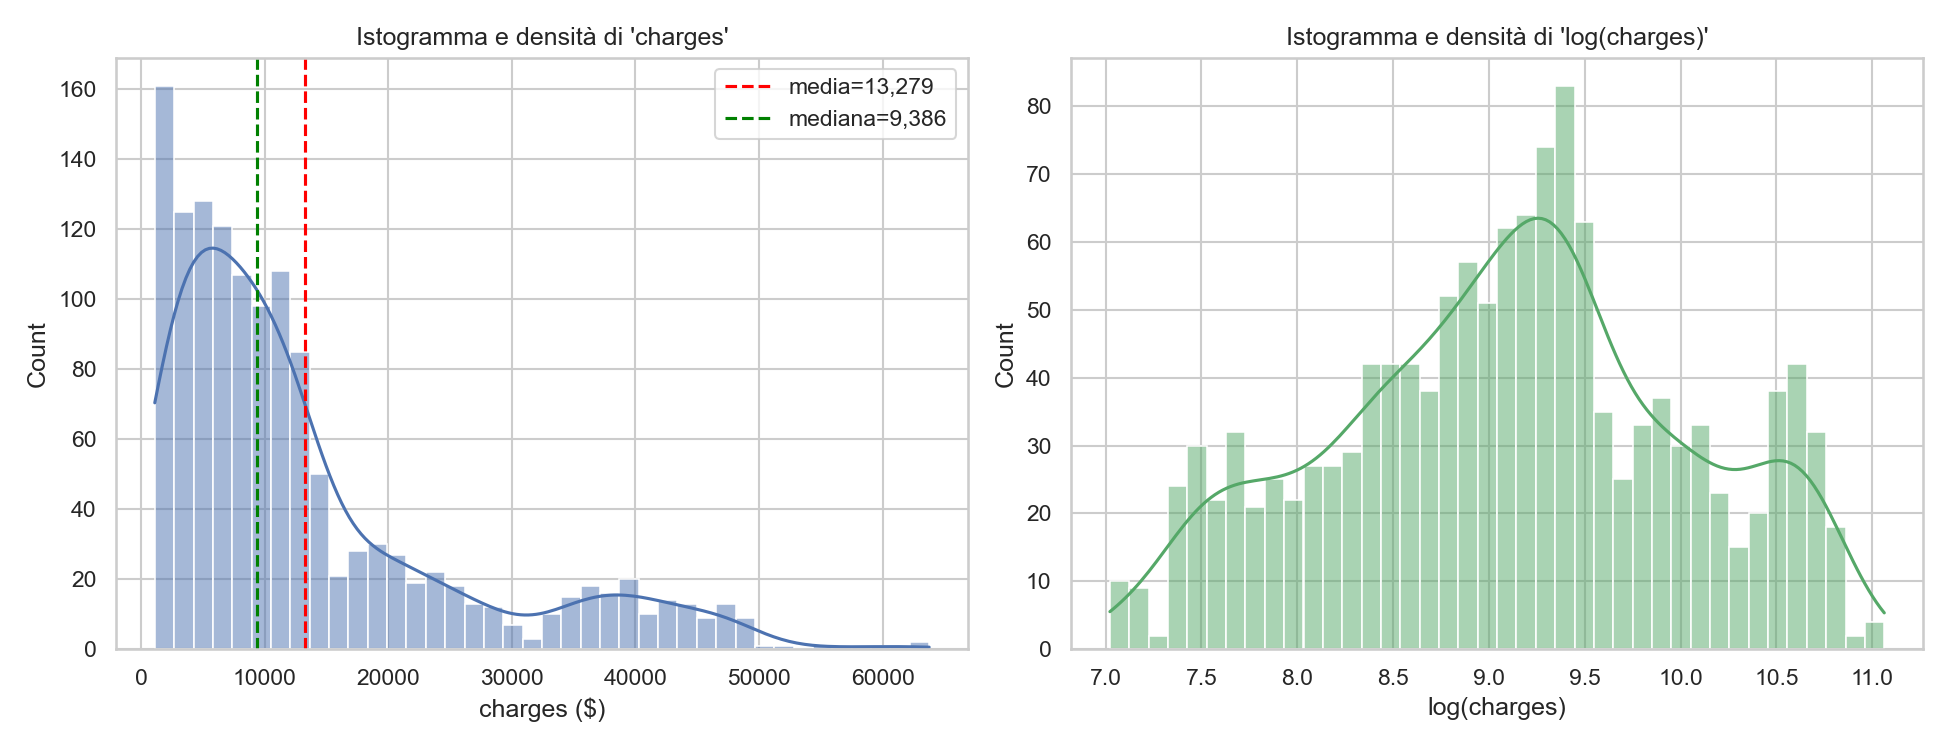
\includegraphics[width=0.95\textwidth]{output/01_charges_distribution.png}
\caption{Istogramma e densità di \texttt{charges} (sinistra) e di
$\log(\texttt{charges})$ (destra).}
\label{fig:dist_charges}
\end{figure}

La Figura~\ref{fig:charges_factors} chiarisce l'origine della bimodalità:
lo stato di fumatore separa nettamente due sotto-popolazioni con spesa
media molto diversa (mediana $\approx\$34\,500$ per i fumatori contro
$\approx\$7\,300$ per i non fumatori), e all'interno di ciascun gruppo la
spesa cresce con età e BMI.

\begin{figure}[H]
\centering
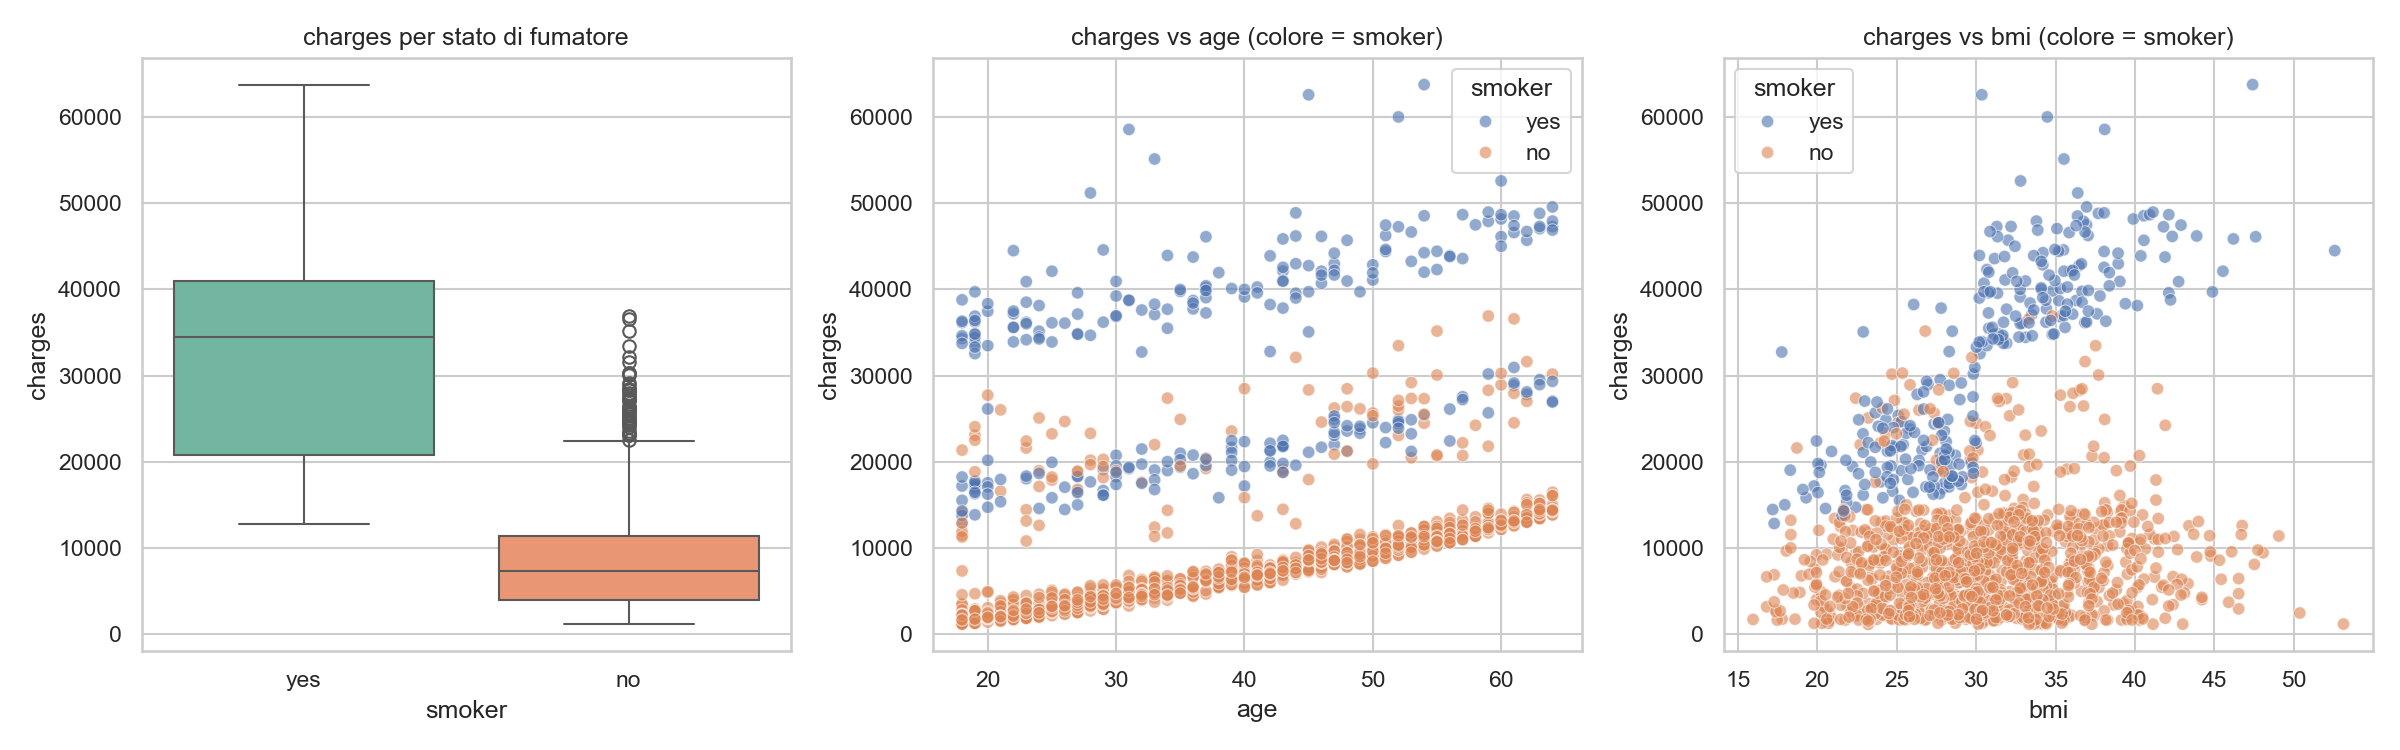
\includegraphics[width=\textwidth]{output/02_charges_by_factors.png}
\caption{\texttt{charges} per stato di fumatore e relazione con
\texttt{age}/\texttt{bmi} colorata per \texttt{smoker}.}
\label{fig:charges_factors}
\end{figure}

\subsection{Matrice di correlazione}
La Figura~\ref{fig:corr} riporta la matrice di correlazione di Pearson tra
tutte le variabili (dopo l'encoding). La correlazione con \texttt{charges}
più forte è quella con \texttt{smoker\_yes} ($\rho=0.787$), seguita da
\texttt{age} ($\rho=0.298$) e \texttt{bmi} ($\rho=0.198$); le altre variabili
mostrano correlazioni deboli ($|\rho|<0.08$). Le correlazioni tra i
regressori sono contenute (il valore assoluto massimo, $0.35$, si osserva
tra le dummy di regione per costruzione), suggerendo a l'assenza di
multicollinearità, ipotesi verificata nella
Sezione~\ref{sec:multicollinearita}.

\begin{figure}[H]
\centering
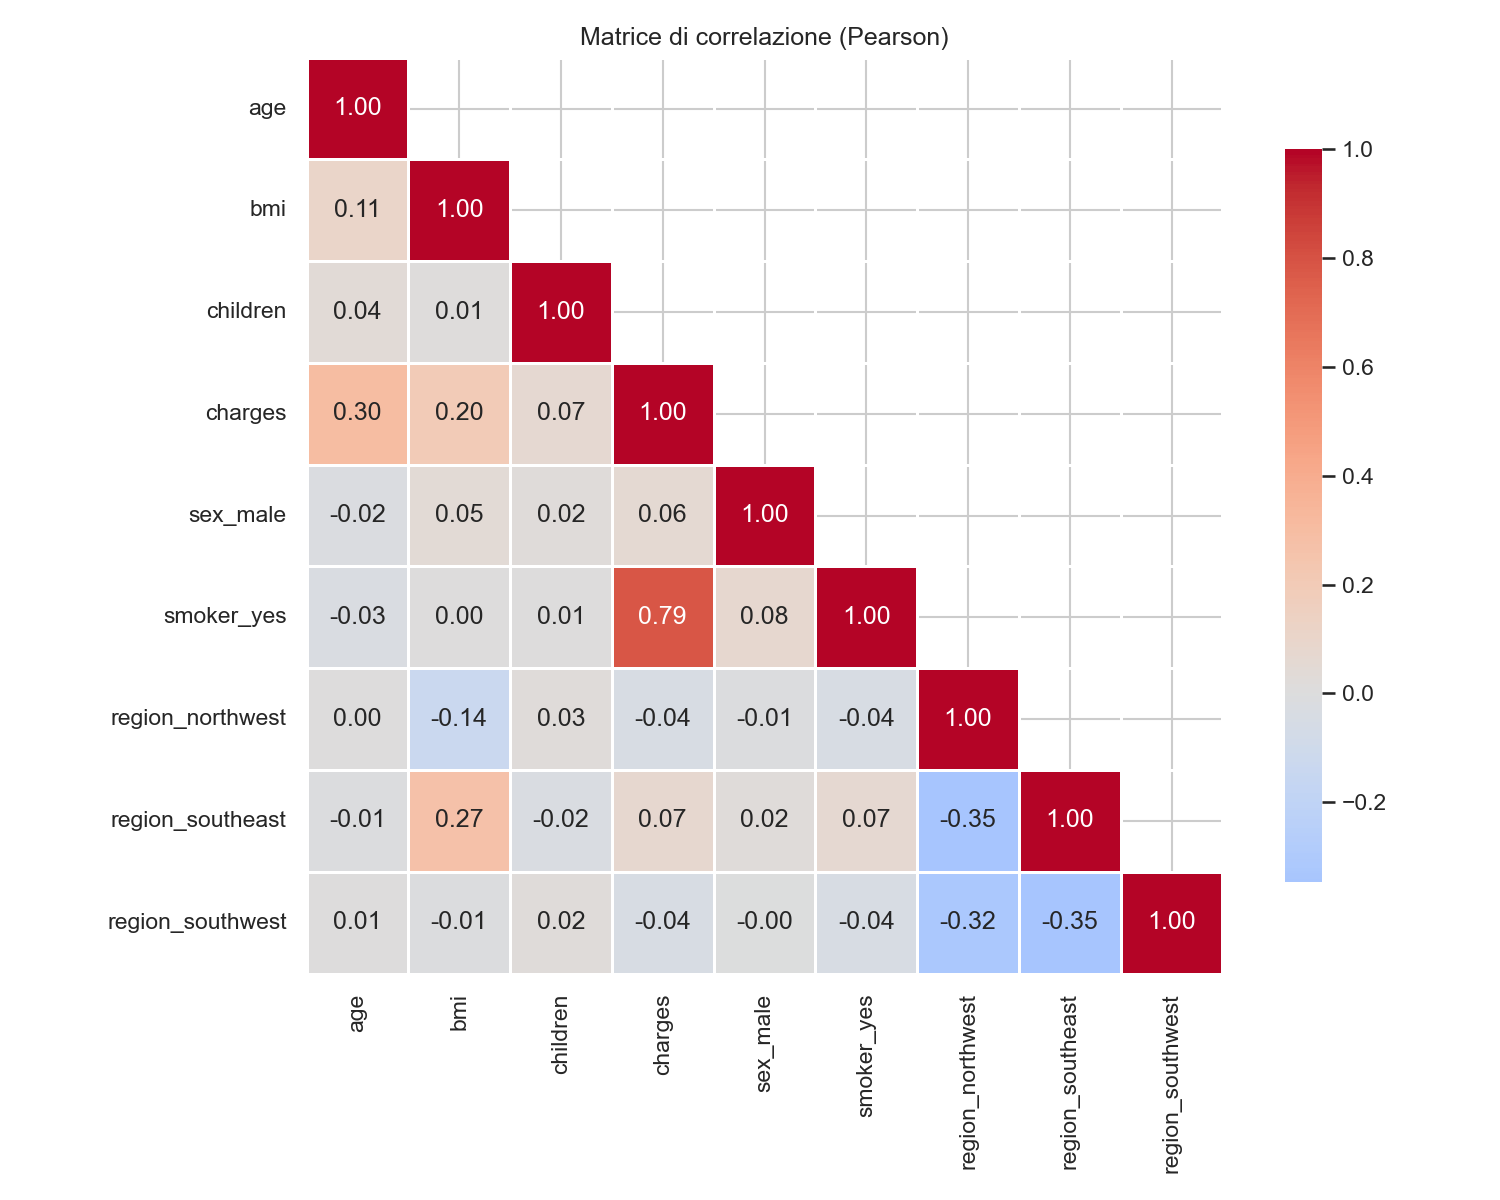
\includegraphics[width=0.75\textwidth]{output/03_correlation_heatmap.png}
\caption{Matrice di correlazione.}
\label{fig:corr}
\end{figure}

\subsection{Matrice di dispersione}
La Figura~\ref{fig:scatter} mostra la scatterplot matrix delle variabili
numeriche con rette di regressione costruite tramite OLS. La relazione
la relazione tra \texttt{age} e \texttt{charges} appare quasi lineare "a strati" (dovuta ai
sottogruppi \texttt{smoker}); quella tra \texttt{bmi} e \texttt{charges} è positiva ma
più rumorosa; quella tra \texttt{children} e \texttt{charges} è pressoché piatta.

\begin{figure}[H]
\centering
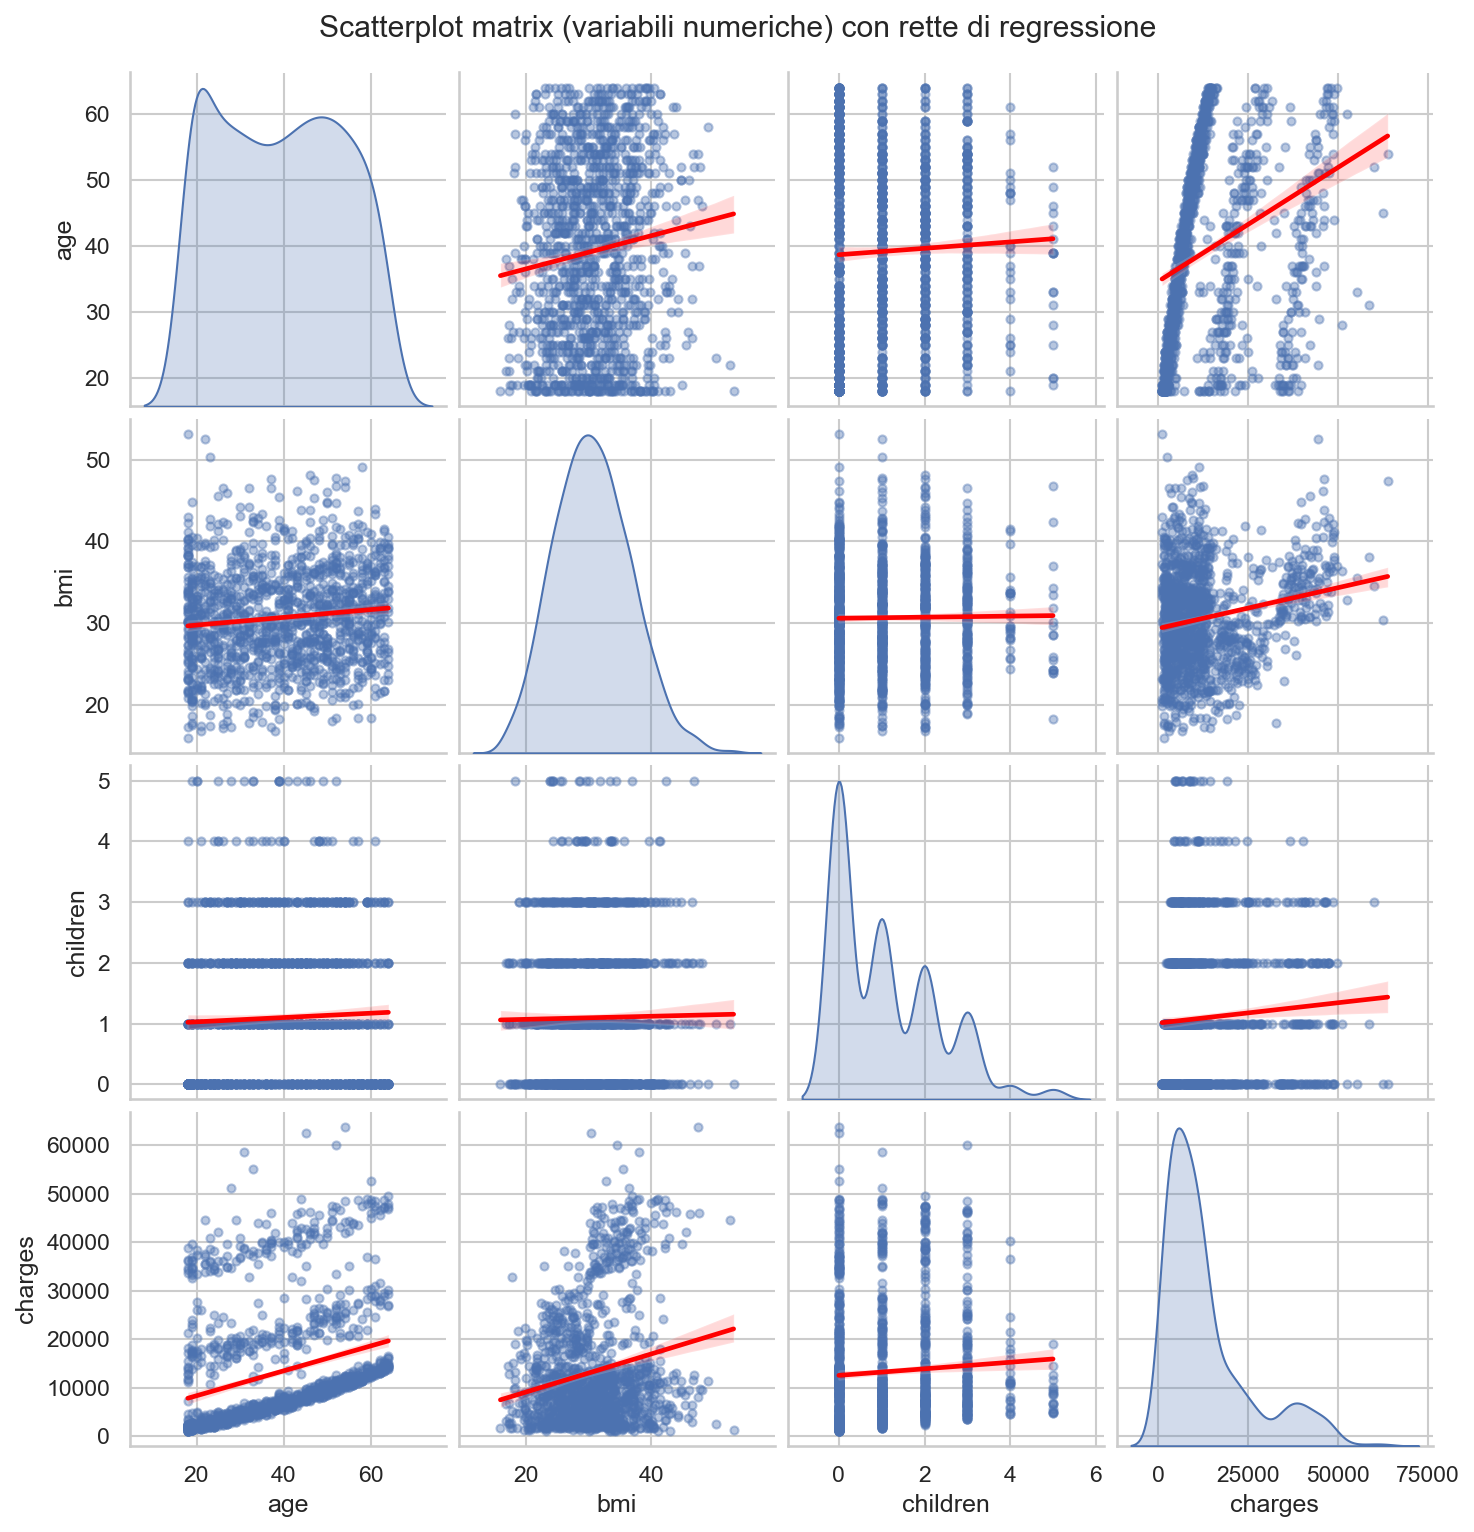
\includegraphics[width=0.85\textwidth]{output/04_scatterplot_matrix.png}
\caption{Scatterplot matrix delle variabili numeriche con rette di
regressione.}
\label{fig:scatter}
\end{figure}

% =======================================================================
\section{Modelli Inferenziali, Forme Funzionali e Multicollinearità}
% =======================================================================

\subsection{Il modello di regressione lineare multipla}
Il modello di partenza (forma lin-lin, tutte le variabili in livelli) è:
\begin{equation}
\texttt{charges}_i = \beta_0 + \beta_1\,\texttt{age}_i + \beta_2\,\texttt{bmi}_i
+ \beta_3\,\texttt{children}_i + \beta_4\,\texttt{sex\_male}_i
+ \beta_5\,\texttt{smoker\_yes}_i + \sum_{r} \gamma_r\,\texttt{region}_{r,i}
+ u_i
\label{eq:modello_completo}
\end{equation}
stimato con il metodo dei minimi quadrati ordinari, sotto le ipotesi di Gauss-Markov ($\mathbb{E}[u_i|X_i]=0$,
$\mathrm{Var}(u_i|X_i)=\sigma^2$, $\mathrm{Cov}(u_i,u_j|X)=0$ per $i\neq j$).

\subsection{Modello completo}
La Tabella~\ref{tab:modello_completo} riporta l'output del modello
\eqref{eq:modello_completo} con tutti gli 8 regressori.

\begin{table}[H]
\centering
\caption{Modello OLS completo (lin-lin): $R^2=0.751$, $R^2_{adj}=0.749$,
$F(8,1328)=500.0$ ($p\approx0$)}
\label{tab:modello_completo}
\begin{tabular}{lrrrrr}
\toprule
Regressore & Coeff. & Std.\,Err. & $t$ & $p$-value & Sign. \\
\midrule
costante           & $-11\,940.0$ & 988.23 & $-12.08$ & $<0.001$ & *** \\
age                & 256.76       & 11.91  & 21.56    & $<0.001$ & *** \\
bmi                & 339.25       & 28.61  & 11.86    & $<0.001$ & *** \\
children           & 474.82       & 137.90 & 3.44     & 0.001    & *** \\
sex\_male          & $-129.48$    & 333.20 & $-0.39$  & 0.698    & n.s. \\
smoker\_yes        & 23\,850.0    & 413.35 & 57.69    & $<0.001$ & *** \\
region\_northwest  & $-349.23$    & 476.82 & $-0.73$  & 0.464    & n.s. \\
region\_southeast  & $-1\,035.27$ & 478.87 & $-2.16$  & 0.031    & * \\
region\_southwest  & $-960.08$    & 478.11 & $-2.01$  & 0.045    & * \\
\bottomrule
\multicolumn{6}{l}{\footnotesize *** $p<0.001$; ** $p<0.01$; * $p<0.05$; n.s. non significativo}
\end{tabular}
\end{table}

I residui del modello completo mostrano forte non-normalità (skewness
$=1.21$, curtosi $=5.65$), un primo
segnale d'allarme che verrà approfondito nella Sezione~\ref{sec:eteroschedasticita}.

\subsection{Confronto dei possibili modelli}
Sono state confrontati quattro modelli: lin-lin, log-log, log-lin e
lin-log:
\begin{align}
\text{lin-lin:} \quad & y = \beta_0 + \boldsymbol{\beta}'\mathbf{x} + u \\
\text{log-log:} \quad & \ln(y) = \beta_0 + \beta_1\ln(\texttt{age}) + \beta_2\ln(\texttt{bmi}) + \boldsymbol{\gamma}'\mathbf{z} + u \\
\text{log-lin:} \quad & \ln(y) = \beta_0 + \boldsymbol{\beta}'\mathbf{x} + u \\
\text{lin-log:} \quad & y = \beta_0 + \beta_1\ln(\texttt{age}) + \beta_2\ln(\texttt{bmi}) + \boldsymbol{\gamma}'\mathbf{z} + u
\end{align}
dove $\mathbf{z}$ raccoglie \texttt{children} e le dummy (che restano sempre
in livelli, poiché il logaritmo non è definito per \texttt{children}=0 e
privo di senso per variabili binarie).

\begin{table}[H]
\centering
\caption{Confronto dei modelli}
\label{tab:forme_funzionali}
\begin{tabular}{lrrrrrr}
\toprule
Forma & $Y$ & $R^2$ & $R^2_{adj}$ & AIC & Skew resid. & Kurt resid. \\
\midrule
lin-lin & charges       & 0.751 & 0.749 & 27\,094.2 & 1.21 & 5.65 \\
log-log & $\ln$(charges) & 0.769 & 0.767 & 1\,627.4  & 1.85 & 7.67 \\
log-lin & $\ln$(charges) & 0.768 & 0.766 & 1\,633.2  & 1.68 & 7.32 \\
lin-log & charges       & 0.744 & 0.743 & 27\,127.8 & 1.18 & 5.45 \\
\bottomrule
\end{tabular}
\end{table}

I valori di $R^2$ e AIC riportati in Tabella~\ref{tab:forme_funzionali}
\textbf{non sono direttamente confrontabili tra le righe con variabile
dipendente diversa} (\texttt{charges} in livelli contro
$\ln(\texttt{charges})$): la varianza totale da spiegare, su cui si basano
sia $R^2$ sia la log-verosimiglianza (e quindi l'AIC), è calcolata su due
scale numeriche differenti. Il confronto è quindi valido solo \emph{entro}
lo stesso gruppo (lin-lin vs.\ lin-log; log-log vs.\ log-lin), non tra i
due gruppi.

La scelta della forma funzionale finale non si basa dunque su un confronto
diretto di questi indici:
\texttt{charges} è una variabile strettamente positiva (supporto
$(0,+\infty)$), trattandosi di una spesa monetaria. Il modello lin-lin,
essendo lineare e non vincolato, può generare previsioni negative, prive
di senso economico: stimato ai valori minimi osservati nel campione
(\texttt{age}=18, \texttt{bmi}=15.96, \texttt{children}=0,
\texttt{smoker\_yes}=0), il modello lin-lin a 4 regressori
(Sezione~\ref{sec:modello_finale}) produce una previsione di
$-\$2\,321.86$, un valore impossibile per una spesa sanitaria.

La trasformazione logaritmica risolve strutturalmente il problema:
$\ln(\texttt{charges})$ ha supporto $(-\infty,+\infty)$, coerente con
l'ipotesi classica dell'errore gaussiano non vincolato
($u_i\sim N(0,\sigma^2)$), e garantisce che le previsioni ritrasformate
$\exp(\widehat{\ln(\texttt{charges})})$ siano sempre positive per
costruzione. Per questo motivo la forma \textbf{log-lin} viene adottata
come specificazione finale nel prosieguo dell'analisi.

\subsection{Selezione del modello: Best Subset Selection}
La scelta del modello finale è stata effettuata tramite \textbf{Best
Subset Selection}: una ricerca esaustiva su tutte le $2^8-1=255$
combinazioni non vuote di regressori (praticabile grazie al basso numero
di regressori disponibili), applicata alla forma log-lin motivata in
Sezione~3.3, selezionando il sottoinsieme che minimizza il criterio BIC
che penalizza la complessità più severamente dell'AIC ed è quindi
preferibile quando l'obiettivo è un modello parsimonioso. Applicata
direttamente a $\ln(\texttt{charges})$ su tutti gli 8 regressori, la
procedura individua come ottimo un modello a 7 regressori (\texttt{age},
\texttt{bmi}, \texttt{children}, \texttt{sex\_male}, \texttt{smoker\_yes},
\texttt{region\_southeast}, \texttt{region\_southwest}; BIC$=1\,676.0$),
poiché in scala logaritmica \texttt{sex\_male} e due dummy di regione
risultano deboli ma statisticamente significative, a differenza di quanto
osservato in scala lin-lin. Per preservare la parsimonia e la
comparabilità con l'estensione con interazione (Sezione~4), si mantiene
tuttavia la specificazione a 4 regressori già individuata nello Step 2:
\begin{equation}
\ln(\texttt{charges}_i) = \beta_0 + \beta_1\,\texttt{age}_i + \beta_2\,\texttt{bmi}_i
+ \beta_3\,\texttt{children}_i + \beta_4\,\texttt{smoker\_yes}_i + u_i
\label{eq:modello_finale}
\end{equation}
il cui BIC ($1\,684.2$) risulta solo marginalmente superiore a quello del
modello a 7 regressori, a fronte di una specificazione più parsimoniosa e
direttamente interpretabile.

\subsection{Analisi del modello finale}
\label{sec:modello_finale}
La Tabella~\ref{tab:modello_finale} riporta l'output completo del modello
log-lin \eqref{eq:modello_finale}.

\begin{table}[H]
\centering
\caption{Modello finale (log-lin, 4 regressori)}
\label{tab:modello_finale}
\begin{tabular}{lrrrrr}
\toprule
Regressore & Coeff. & Std.\,Err. & $t$ & $p$-value & IC 95\% \\
\midrule
costante    & 6.9850 & 0.070 & 100.17 & $<0.001$ & $[6.848,\,7.122]$ \\
age         & 0.0347 & 0.001 & 39.43  & $<0.001$ & $[0.033,\,0.037]$ \\
bmi         & 0.0106 & 0.002 & 5.24   & $<0.001$ & $[0.007,\,0.015]$ \\
children    & 0.1009 & 0.010 & 9.89   & $<0.001$ & $[0.081,\,0.121]$ \\
smoker\_yes & 1.5427 & 0.030 & 50.69  & $<0.001$ & $[1.483,\,1.602]$ \\
\bottomrule
\end{tabular}
\end{table}

\textbf{Bontà di adattamento:} $R^2=0.762$, $R^2_{adj}=0.761$: il modello
spiega il 76.2\% della varianza di $\ln(\texttt{charges})$.

\textbf{Test $F$ globale:} verifica la significatività congiunta di tutti
i regressori ($H_0:\beta_1=\dots=\beta_k=0$). Si ottiene
$F(4,1332)=1065.2$, $p\approx0$: si rigetta $H_0$, il modello nel
suo complesso è significativo.

\textbf{Test $t$ sui singoli coefficienti} ($H_0:\beta_j=0$ vs.\
$H_1:\beta_j\neq0$, statistica $t=\hat\beta_j/\mathrm{SE}(\hat\beta_j)$):
tutti e 4 i regressori sono significativi. In forma log-lin i coefficienti
si interpretano in termini di percentuali: $(\exp(\hat\beta_j)-1)\times100$
è la variazione percentuale attesa di \texttt{charges} per un incremento
unitario di $x_j$, a parità delle altre covariate. Un anno di età in più è
associato a una variazione attesa della spesa di $+3.5\%$; un punto di BMI
in più a $+1.1\%$; un figlio in più a $+10.6\%$; essere fumatori a
$+367.7\%$ ($(\exp(1.5427)-1)\times100$), effetto di gran lunga
dominante, coerente con la correlazione $\rho=0.787$ osservata in Sez.~2.

\subsection{Multicollinearità}
\label{sec:multicollinearita}
Il \textbf{Variance Inflation Factor} per il regressore $j$ è definito come
\begin{equation}
\mathrm{VIF}_j = \frac{1}{1-R_j^2}
\end{equation}
dove $R_j^2$ è il coefficiente di determinazione della regressione di
$x_j$ su tutti gli altri regressori. La Tabella~\ref{tab:vif} riporta i VIF
del modello finale.

\begin{table}[H]
\centering
\caption{Variance Inflation Factor, modello finale}
\label{tab:vif}
\begin{tabular}{lr}
\toprule
Regressore & VIF \\
\midrule
age        & 1.014 \\
bmi        & 1.012 \\
children   & 1.002 \\
smoker\_yes & 1.001 \\
\bottomrule
\end{tabular}
\end{table}

Tutti i VIF sono prossimi a 1 (soglia di allarme convenzionale:
$\mathrm{VIF}\geq10$): nessuna
multicollinearità rilevante tra i regressori.

Come indicatore complementare è stato calcolato il \textbf{Condition
Number} $k$ della matrice disegno $X$ (inclusa la costante), definito
semplicemente come la radice quadrata del rapporto tra l'autovalore
massimo e l'autovalore minimo della matrice $X'X$:
\begin{equation}
k = \sqrt{\frac{\lambda_{max}(X'X)}{\lambda_{min}(X'X)}}
\end{equation}
Si ottiene $k=291.6$ (soglie di riferimento: $k<10$ nessun problema,
$10\leq k<30$ moderato, $k\geq30$ severo). Il valore elevato è in larga
parte attribuibile alla diversa scala di misura dei regressori (age e bmi
assumono valori nell'ordine delle decine, mentre le dummy sono 0/1),
piuttosto che a una reale relazione lineare tra le variabili: coerentemente,
tutti i VIF restano prossimi a 1. Poiché il VIF non risente della scala
delle variabili, viene qui considerato l'indicatore più affidabile per la
diagnosi di multicollinearità.
\textbf{Conclusione}: nessun problema di multicollinearità rilevante nel
modello finale.

% =======================================================================
\section{Eteroschedasticità e Analisi dei Residui}
\label{sec:eteroschedasticita}
% =======================================================================

\subsection{Analisi grafica}
La Figura~\ref{fig:resid_fitted} mostra i residui del modello log-lin
finale \eqref{eq:modello_finale} (in scala logaritmica) contro i valori
stimati, colorati per stato di fumatore. Anche in scala logaritmica si
osservano due nubi nettamente separate, ciascuna con un andamento non
lineare, sintomo di eteroschedasticità residua e di una possibile
interazione \texttt{smoker}$\times$\texttt{bmi} non ancora modellata.

\begin{figure}[H]
\centering
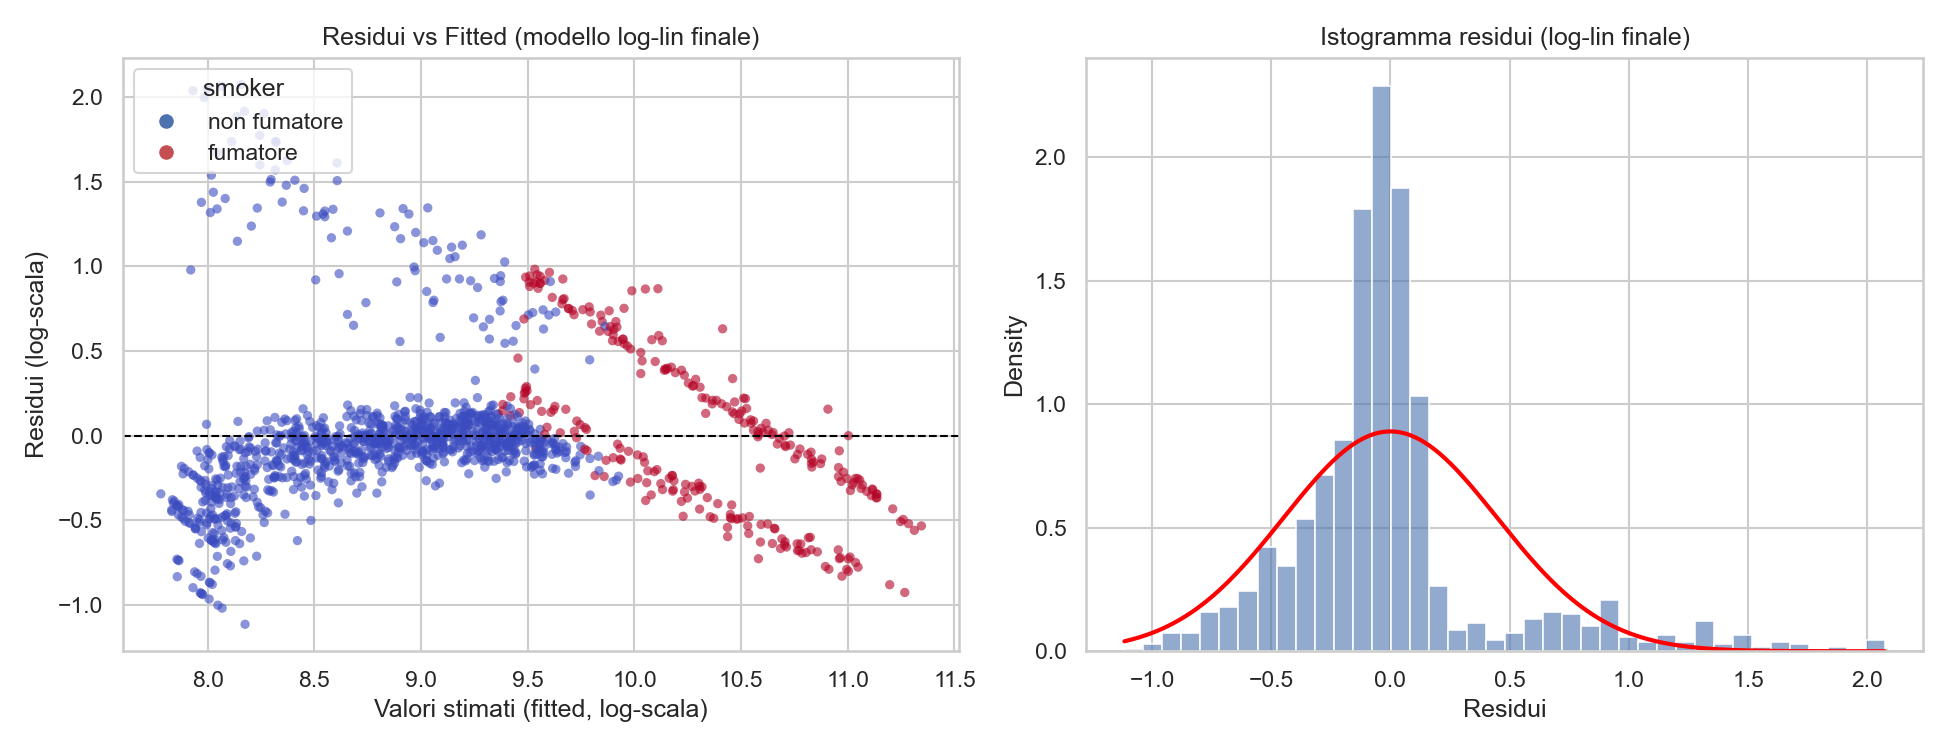
\includegraphics[width=\textwidth]{output/16_residuals_loglin_final.png}
\caption{Residui vs.\ Fitted values (colorati per \texttt{smoker}) e
istogramma dei residui con densità normale teorica sovrapposta, modello
log-lin finale.}
\label{fig:resid_fitted}
\end{figure}

Il Q-Q plot (Figura~\ref{fig:qqplot}) conferma code pesanti e uno
scostamento dalla normalità, sebbene meno marcato che in scala lineare.

\begin{figure}[H]
\centering
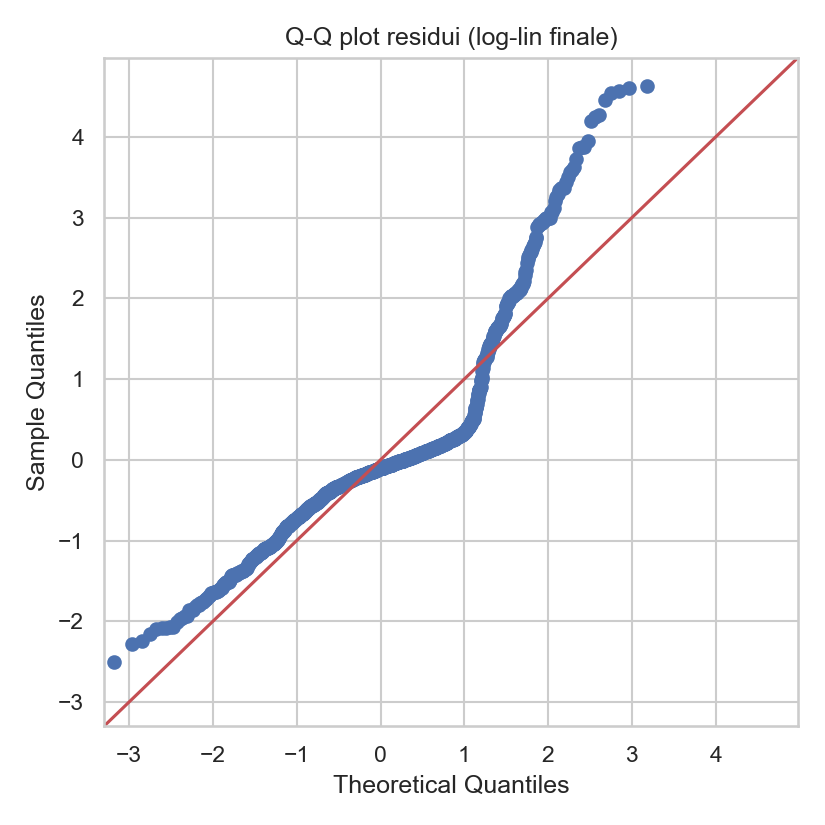
\includegraphics[width=0.55\textwidth]{output/17_qqplot_loglin_final.png}
\caption{Q-Q plot dei residui del modello log-lin finale.}
\label{fig:qqplot}
\end{figure}

\subsection{Test di Breusch-Pagan e White}
Il test di \textbf{Breusch-Pagan} verifica $H_0: \mathrm{Var}(u_i|X_i)=\sigma^2$
(omoschedasticità) contro $H_1$: la varianza dipende linearmente dai
regressori, tramite la regressione ausiliaria
$\hat{u}_i^2 = \delta_0+\delta_1 x_{1i}+\dots+\delta_k x_{ki}+v_i$ e la
statistica $\mathrm{LM}=nR^2_{aux}\sim\chi^2_k$. Il test di \textbf{White}
generalizza includendo nella regressione ausiliaria anche quadrati e
prodotti incrociati dei regressori, risultando robusto a forme di
eteroschedasticità non lineari.

\begin{table}[H]
\centering
\caption{Test di eteroschedasticità sul modello log-lin finale}
\label{tab:bp_white}
\begin{tabular}{lrrrr}
\toprule
Test & Statistica & $p$-value & Statistica $F$ & $p$-value ($F$) \\
\midrule
Breusch-Pagan & LM$=81.23$  & $9.56\times10^{-17}$ & 21.54 & $3.08\times10^{-17}$ \\
White         & LM$=140.86$ & $1.41\times10^{-23}$ & 11.99 & $5.47\times10^{-25}$ \\
\bottomrule
\end{tabular}
\end{table}

Entrambi i test rigettano nettamente $H_0$ ($p<0.001$):
\textbf{eteroschedasticità confermata anche in scala logaritmica}. La
trasformazione log, pur risolvendo il problema della non negatività delle
previsioni (Sezione 3.3), non garantisce di per sé varianza costante dei
residui.

\subsection{Rimedio 1: inclusione del termine di interazione smoker $\times$ bmi}
L'analisi esplorativa (Sezione 2) e il pattern osservato nei residui (Sezione
4.1) suggeriscono che l'effetto di \texttt{bmi} su \texttt{charges} non sia
lo stesso per fumatori e non fumatori. Si stima quindi un modello log-lin
esteso che include il termine di interazione \texttt{smoker\_yes} $\times$
\texttt{bmi}:
\begin{equation}
\ln(\texttt{charges}_i) = \beta_0 + \beta_1\,\texttt{age}_i + \beta_2\,\texttt{bmi}_i
+ \beta_3\,\texttt{children}_i + \beta_4\,\texttt{smoker\_yes}_i
+ \beta_5\,(\texttt{smoker\_yes}_i \times \texttt{bmi}_i) + u_i
\label{eq:modello_interazione}
\end{equation}

\begin{table}[H]
\centering
\caption{Modello log-lin con interazione smoker $\times$ bmi}
\label{tab:interazione}
\begin{tabular}{lrrrr}
\toprule
Regressore & Coeff. & Std.\,Err. & $t$ & $p$-value \\
\midrule
costante                        & 7.2740  & 0.074  & 97.94  & $<0.001$ \\
age                             & 0.0350  & 0.001  & 40.94  & $<0.001$ \\
bmi                             & 0.0009  & 0.002  & 0.39   & 0.695 \\
children                        & 0.1020  & 0.010  & 10.32  & $<0.001$ \\
smoker\_yes                     & 0.1859  & 0.148  & 1.26   & 0.209 \\
smoker\_yes $\times$ bmi        & 0.0442  & 0.005  & 9.37   & $<0.001$ \\
\bottomrule
\end{tabular}
\end{table}

\textbf{Bontà di adattamento:} $R^2=0.777$ e $R^2_{adj}=0.776$, contro
$R^2=0.762$ e $R^2_{adj}=0.761$ del modello senza interazione. Il test $F$ incrementale tra il modello conferma la significatività
congiunta dell'aggiunta: $F(1,1331)=87.8$, $p\approx3.03\times10^{-20}$, in
linea con il test $t$ sul singolo coefficiente ($t=9.37$, $p<0.001$).
L'interazione è quindi altamente significativa.

\textbf{Interpretazione:} l'effetto marginale di
\texttt{bmi} risulta diverso nei due gruppi. Per i non
fumatori, $(\exp(\hat\beta_2)-1)\times100 = +0.09\%$ per punto di BMI,
non significativo ($p=0.695$); per i fumatori, sommando i coefficienti
($\hat\beta_2+\hat\beta_5=0.0451$, $t=10.81$, $p<0.001$),
$(\exp(0.0451)-1)\times100 = +4.61\%$ per punto di BMI, un effetto significativo. Questo spiega precisamente il pattern
quasi discontinuo osservato nello Step 1 (Figura~\ref{fig:charges_factors}):
l'obesità amplifica sensibilmente i costi sanitari specificamente nei
fumatori, mentre per i non fumatori il BMI ha un effetto marginale quasi
nullo sulla spesa a parità di età e figli.

Di conseguenza anche i coefficienti principali di \texttt{bmi} e
\texttt{smoker\_yes} cambiano interpretazione: rappresentano il valore
stimato quando l'altra variabile coinvolta nell'interazione è pari a
zero, non più un effetto medio costante. In particolare
\texttt{smoker\_yes} ora rappresenta l'effetto di essere fumatori quando
\texttt{bmi}=0, un valore fuori dal range osservato (da 15.96 a 53.13) e
privo di senso diretto (coerentemente non significativo, $p=0.209$).
L'effetto complessivo del fumo, calcolato al BMI medio del campione
($\overline{\texttt{bmi}}=30.66$; $t=52.27$, $p<0.001$), è
$(\exp(0.1859+0.0442\times30.66)-1)\times100 \approx +367\%$, coerente
con la stima $+367.7\%$ del modello senza interazione.

\begin{table}[H]
\centering
\caption{Variance Inflation Factor, modello con interazione}
\label{tab:vif_interazione}
\begin{tabular}{lr}
\toprule
Regressore & VIF \\
\midrule
age                       & 1.015 \\
bmi                       & 1.297 \\
children                  & 1.002 \\
smoker\_yes                & 25.14 \\
smoker\_yes $\times$ bmi   & 25.44 \\
\bottomrule
\end{tabular}
\end{table}

Il VIF (indipendente dalla scala di \texttt{charges}, poiché dipende solo
dalla matrice dei regressori $X$) evidenzia una collinearità elevata tra
\texttt{smoker\_yes} e il termine di interazione (VIF $\approx25$),
conseguenza meccanica dell'uso di \texttt{bmi} non centrata: nel
sottogruppo dei fumatori, \texttt{smoker\_yes}$\times$\texttt{bmi} è
quasi proporzionale a \texttt{bmi} stessa. Questo non compromette la
validità del modello (i coefficienti restano stimati correttamente e il
termine di interazione resta altamente significativo), ma riduce la
precisione con cui si può scomporre l'effetto tra i due termini correlati;
centrando \texttt{bmi} sulla propria media si ridurrebbe il VIF senza
alterare fit, $R^2$ o significatività, a scapito della diretta
interpretabilità dei coefficienti principali in corrispondenza di
\texttt{bmi}=0.

\begin{table}[H]
\centering
\caption{Confronto dei test di eteroschedasticità: senza vs. con interazione (log-lin)}
\label{tab:bp_white_interazione}
\begin{tabular}{lrrrr}
\toprule
Test & LM senza interazione & $p$-value & LM con interazione & $p$-value \\
\midrule
Breusch-Pagan & 81.23 & $9.56\times10^{-17}$ & 76.57  & $4.37\times10^{-15}$ \\
White         & 140.86 & $1.41\times10^{-23}$ & 129.74 & $7.21\times10^{-20}$ \\
\bottomrule
\end{tabular}
\end{table}

A differenza di quanto accadrebbe in scala lin-lin, dove l'interazione
elimina l'eteroschedasticità (i due test tornerebbero non significativi),
in scala log-lin \textbf{entrambi i test restano altamente significativi}
anche dopo l'inclusione dell'interazione: la statistica LM di
Breusch-Pagan si riduce solo del 5.7\% (da 81.23 a 76.57) e quella di
White del 7.9\% (da 140.86 a 129.74), entrambe ancora con $p<0.001$.
L'interazione migliora quindi in modo sostanziale il fit del modello, ma
\textbf{non risolve} l'eteroschedasticità nella specificazione log-lin: la
trasformazione logaritmica ha già assorbito gran parte della relazione
media-varianza, lasciando un margine di correzione residuo minore rispetto
alla specificazione in livelli.

\begin{figure}[H]
\centering
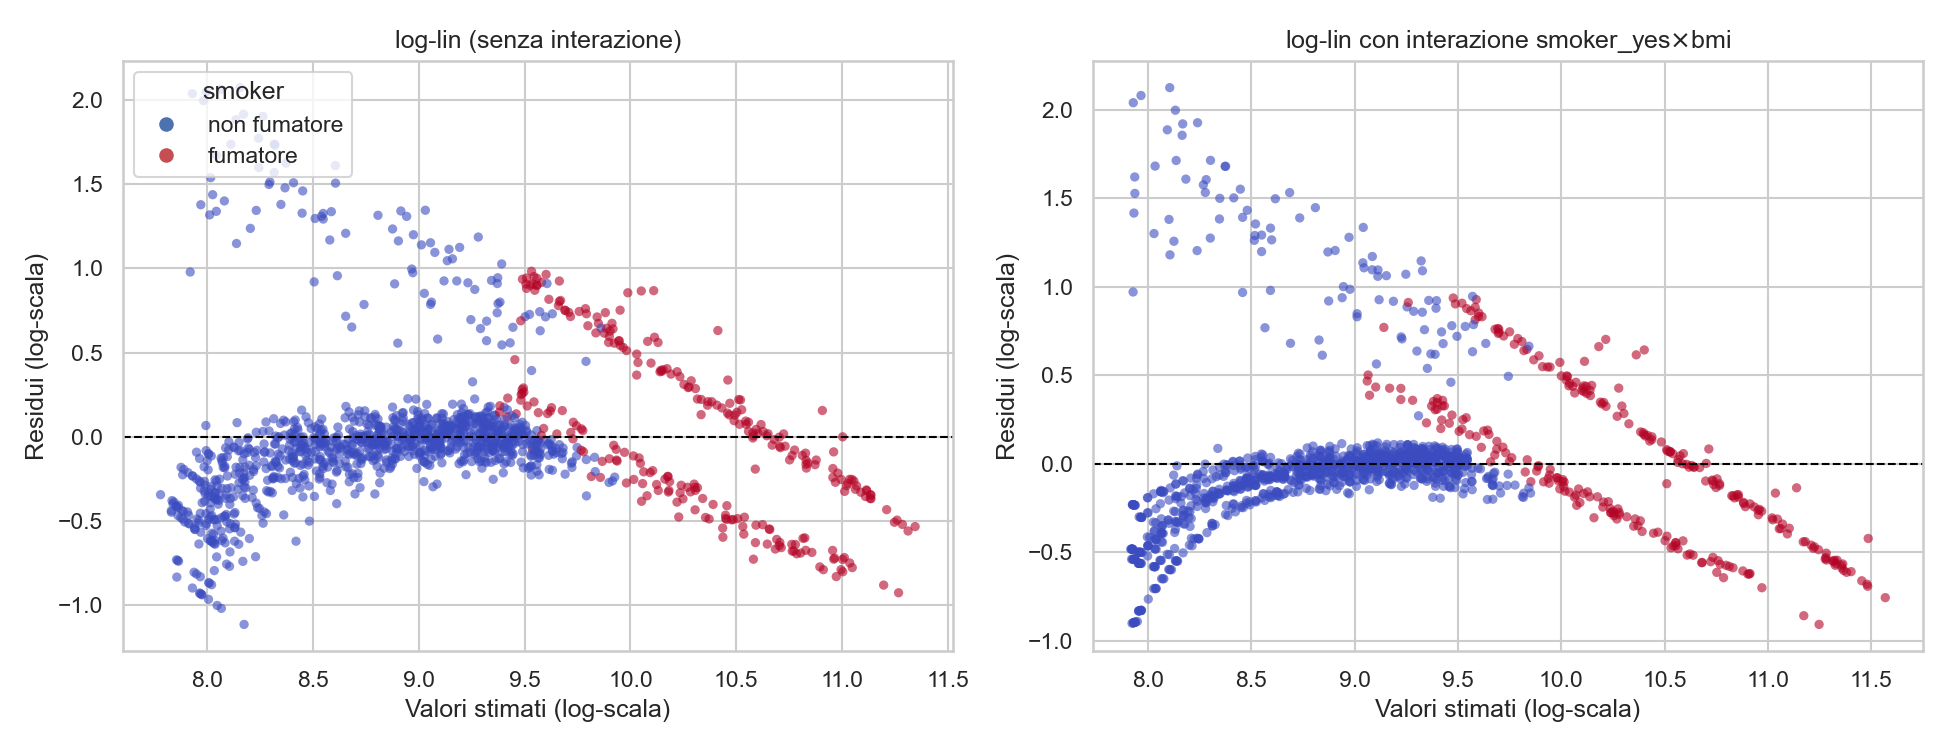
\includegraphics[width=\textwidth]{output/18_residuals_loglin_interaction_comparison.png}
\caption{Confronto Residui vs Fitted (scala logaritmica): modello senza
interazione (sinistra) e con interazione \texttt{smoker\_yes}$\times$\texttt{bmi}
(destra), colorati per \texttt{smoker}.}
\label{fig:resid_interaction}
\end{figure}

Il pannello destro mostra come, per i non fumatori, la nube dei residui si
restringa e assuma un andamento più regolare per bassi valori stimati; per
i fumatori la dispersione decrescente resta ben visibile, coerente con la
persistenza dell'eteroschedasticità rilevata dai test.

Va inoltre notato che skewness e curtosi dei residui aumentano leggermente
nel modello con interazione (skewness $1.60\to1.76$, curtosi
$7.18\to7.80$).

\subsection{Rimedio 2: Modello Lineare Robusto (RLM)}
Il Modello Lineare Robusto (RLM) è stato applicato al modello log-lin
finale (senza interazione), come ulteriore strumento diagnostico
indipendente dalla specificazione adottata, per verificare quanto le
osservazioni anomale (outlier) influenzino le stime OLS: a differenza dei
minimi quadrati ordinari, l'RLM attribuisce un peso $w_i<1$ alle
osservazioni con residuo elevato, riducendone l'impatto sulla stima dei
coefficienti.

\begin{table}[H]
\centering
\caption{Confronto coefficienti (log-lin) e semi-elasticità: OLS vs.\ RLM}
\label{tab:rlm}
\begin{tabular}{lrrrr}
\toprule
Regressore & OLS & Semi-elast.\ OLS & RLM & Semi-elast.\ RLM \\
\midrule
costante    & 6.9850 & --            & 6.9442 & -- \\
age         & 0.0347 & $+3.5\%$      & 0.0398 & $+4.1\%$ \\
\textbf{bmi} & \textbf{0.0106} & \textbf{$+1.1\%$} & \textbf{0.0030} & \textbf{$+0.3\%$} \\
children    & 0.1009 & $+10.6\%$     & 0.1020 & $+10.7\%$ \\
\textbf{smoker\_yes} & \textbf{1.5427} & \textbf{$+367.7\%$} & \textbf{1.5709} & \textbf{$+381.1\%$} \\
\bottomrule
\end{tabular}
\end{table}

L'RLM assegna un peso molto basso a un insieme di osservazioni anomale,
in questo caso prevalentemente soggetti giovani e non fumatori con
\texttt{charges} elevate rispetto al proprio profilo (verosimilmente per
fattori di rischio non osservati nel dataset). Rispetto all'OLS, l'RLM
stima un effetto di \texttt{bmi} più contenuto (semi-elasticità:
$+1.1\%\to+0.3\%$ per punto) e un effetto di \texttt{age} e
\texttt{smoker\_yes} leggermente più marcato ($+3.5\%\to+4.1\%$ e
$+367.7\%\to+381.1\%$): alcuni outlier attenuano nell'OLS classico
l'effetto di età e fumo, effetto che l'RLM restituisce con maggiore
fedeltà una volta ridotto il loro peso.

\begin{figure}[H]
\centering
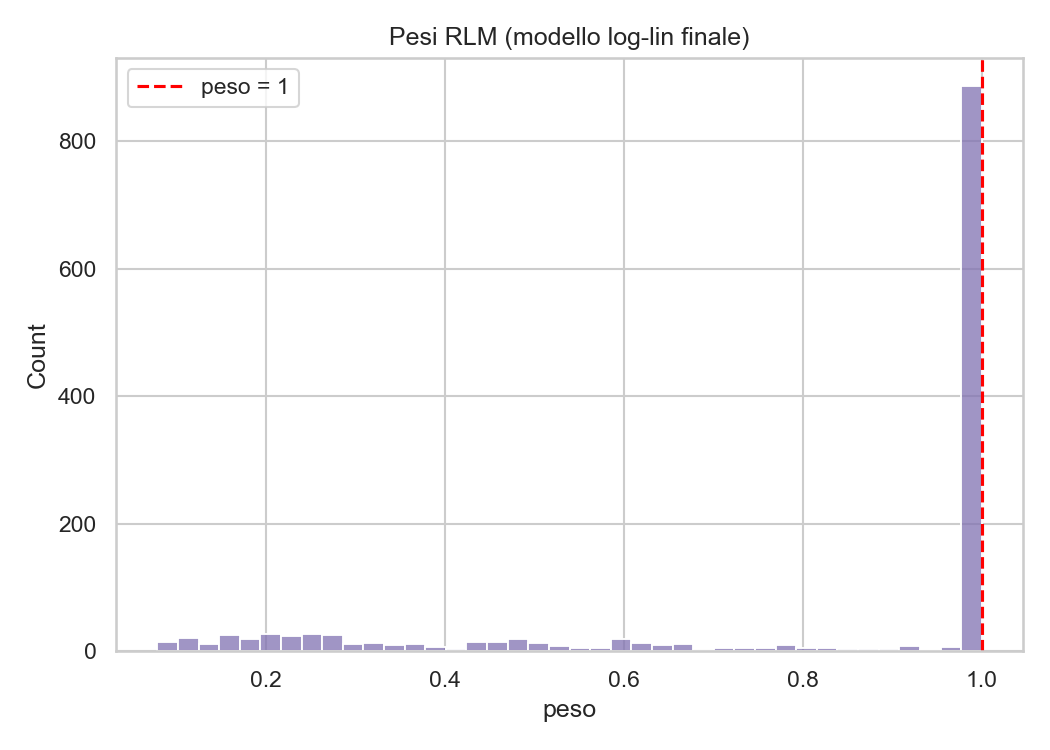
\includegraphics[width=0.6\textwidth]{output/19_rlm_weights_loglin.png}
\caption{Distribuzione dei pesi assegnati dal Modello Lineare Robusto
(modello log-lin finale).}
\label{fig:rlm_weights}
\end{figure}

\subsection{Sintesi}
Nella specificazione log-lin adottata come modello finale,
l'eteroschedasticità rilevata in Sezione 4.2 (Breusch-Pagan e White,
$p<0.001$) persiste anche dopo l'inclusione del termine di interazione
\texttt{smoker\_yes}$\times$\texttt{bmi} (Rimedio 1): l'interazione
migliora significativamente il fit ($R^2$ da 0.762 a 0.777) ma riduce le
statistiche LM solo del tra il 5.7\% e il 7.9\%, che restano altamente significative.
La trasformazione logaritmica, avendo già stabilizzato gran parte della
relazione media-varianza, lascia dunque un margine di correzione residuo
minore rispetto alla specificazione in livelli, dove lo stesso termine di
interazione elimina l'eteroschedasticità. Il Modello Lineare Robusto
(Rimedio 2) conferma che alcune osservazioni anomale distorcono le stime
OLS, in particolare quella di \texttt{bmi}. Data la persistenza
dell'eteroschedasticità, l'uso di errori standard robusti resta
comunque utile per un'inferenza valida sui coefficienti del
modello log-lin finale.

% =======================================================================
\section{Modelli Predittivi: Regolarizzazione}
% =======================================================================

\subsection{Impostazione}
A differenza degli Step precedenti, in questa sezione si utilizzano
\textbf{tutti gli 8 regressori} codificati, lasciando che siano le
tecniche di regolarizzazione a operare la selezione/riduzione delle
variabili in modo automatico. Il campione è stato suddiviso in training
(80\%, $n=1069$) e test set (20\%, $n=268$); i regressori continui
(\texttt{age}, \texttt{bmi}, \texttt{children}) sono stati standardizzati
($z=(x-\bar x)/s$, scaler stimato solo sul training set per evitare
\emph{data leakage}), mentre le dummy restano in scala 0/1.

Le tre famiglie di modelli risolvono:
\begin{align}
\text{Ridge:} \quad & \hat{\boldsymbol\beta}_{Ridge} = \arg\min_{\boldsymbol\beta} \left\{ \mathrm{SSE} + \lambda\sum_{j=1}^k \beta_j^2 \right\} \\
\text{LASSO:} \quad & \hat{\boldsymbol\beta}_{LASSO} = \arg\min_{\boldsymbol\beta} \left\{ \mathrm{SSE} + \lambda\sum_{j=1}^k |\beta_j| \right\} \\
\text{Elastic Net:} \quad & \hat{\boldsymbol\beta}_{EN} = \arg\min_{\boldsymbol\beta} \left\{ \mathrm{SSE} + \lambda\Big[\alpha\sum_{j=1}^k |\beta_j| + \tfrac{1-\alpha}{2}\sum_{j=1}^k \beta_j^2\Big] \right\}
\end{align}
dove $\lambda\geq0$ è il parametro di regolarizzazione e
$\alpha\in[0,1]$ pesa il
contributo relativo delle penalità L1/L2 (testati $\alpha=0.1$, a
prevalenza Ridge, e $\alpha=0.9$, a prevalenza LASSO).

È stata definita una griglia logaritmica decrescente di 100 valori,
$\lambda\in\{10^{4},\dots,10^{-4}\}$, e per ciascun valore è stata
eseguita una \textbf{10-fold cross-validation} sul training set.

\subsection{Trace plot dei coefficienti}
La Figura~\ref{fig:trace} mostra i \emph{trace plot}: per $\lambda$ grande
tutti i coefficienti sono schiacciati verso 0; al decrescere di $\lambda$
(verso destra, asse $-\log_{10}\lambda$) "si accendono" in ordine di
importanza, con \texttt{smoker\_yes} dominante seguito da \texttt{age} e
\texttt{bmi}. Nel pannello LASSO si osserva la differenza qualitativa
attesa rispetto a Ridge/Elastic Net: le variabili deboli (\texttt{sex\_male}
e le dummy di \texttt{region}) restano \textbf{esattamente a zero} per un
ampio intervallo di $\lambda$, mentre con la penalità L2 si
avvicinano a zero senza mai annullarsi.

\begin{figure}[H]
\centering
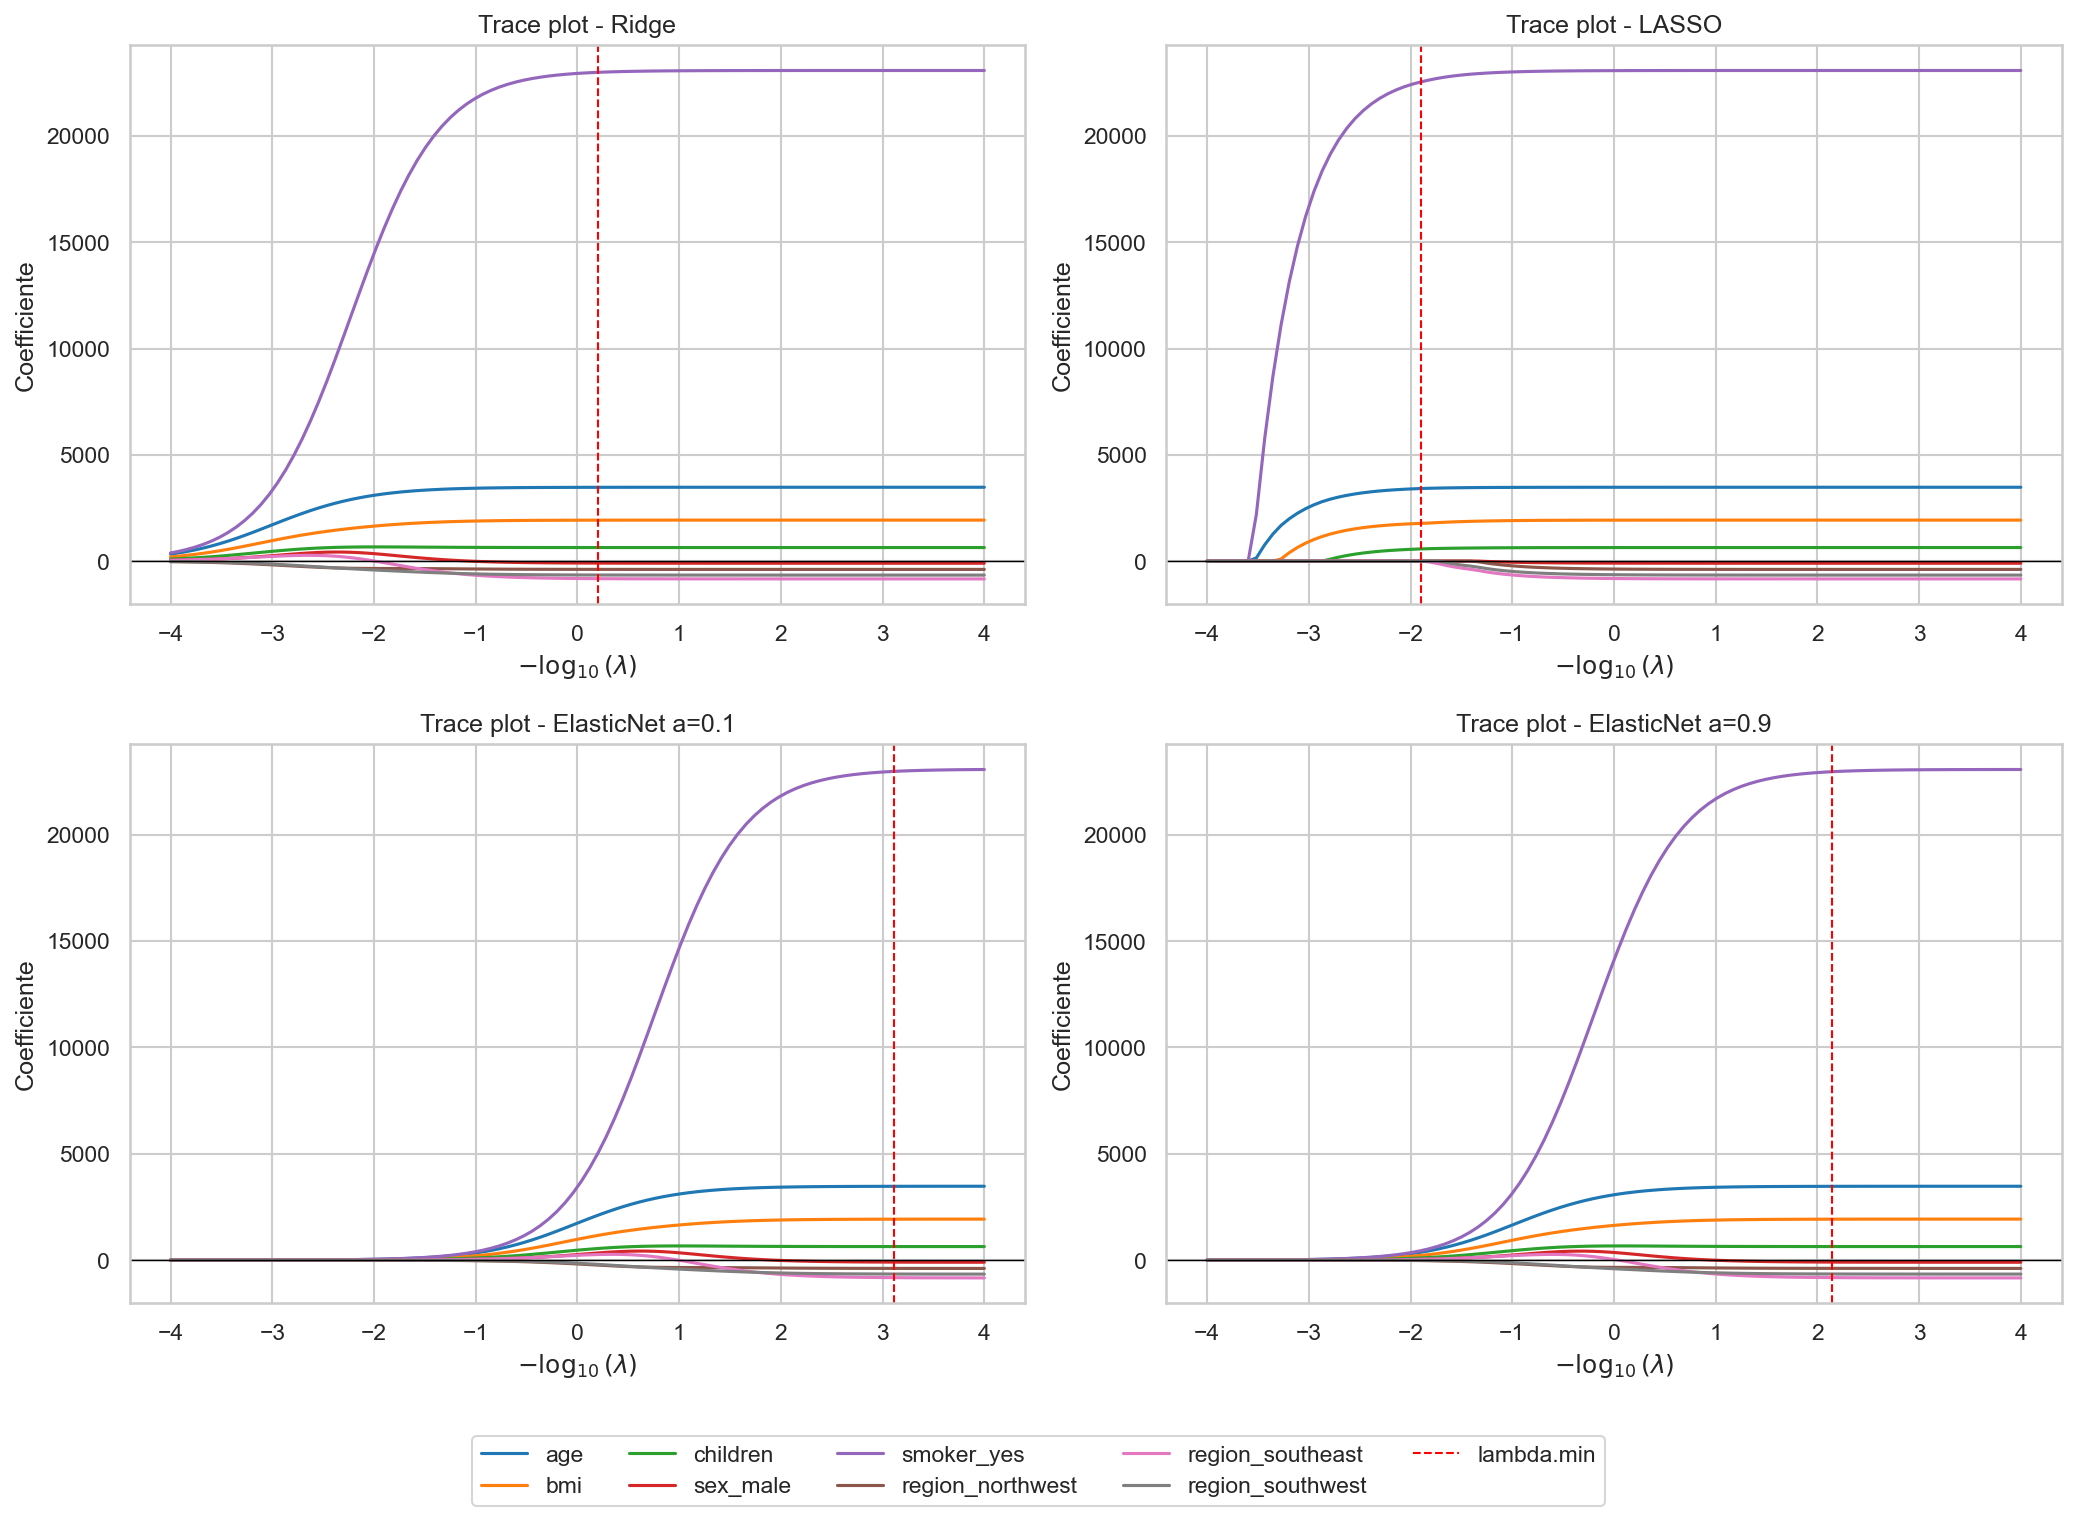
\includegraphics[width=\textwidth]{output/11_trace_plots.png}
\caption{Trace plot dei coefficienti in funzione di $-\log_{10}(\lambda)$.}
\label{fig:trace}
\end{figure}

\subsection{Cross-Validation: MSE vs.\ $-\log(\lambda)$}
La Figura~\ref{fig:cvmse} mostra le curve di CV-MSE (media $\pm$ errore
standard sui 10 fold) in funzione di $-\log_{10}(\lambda)$. Il parametro
di regolarizzazione ottimale $\lambda_{min}$ è individuato come il valore
che minimizza il CV-MSE medio sui 10 fold, evidenziato nel grafico da una
linea verticale: è questo l'unico criterio adottato per la scelta di
$\lambda$.

\begin{figure}[H]
\centering
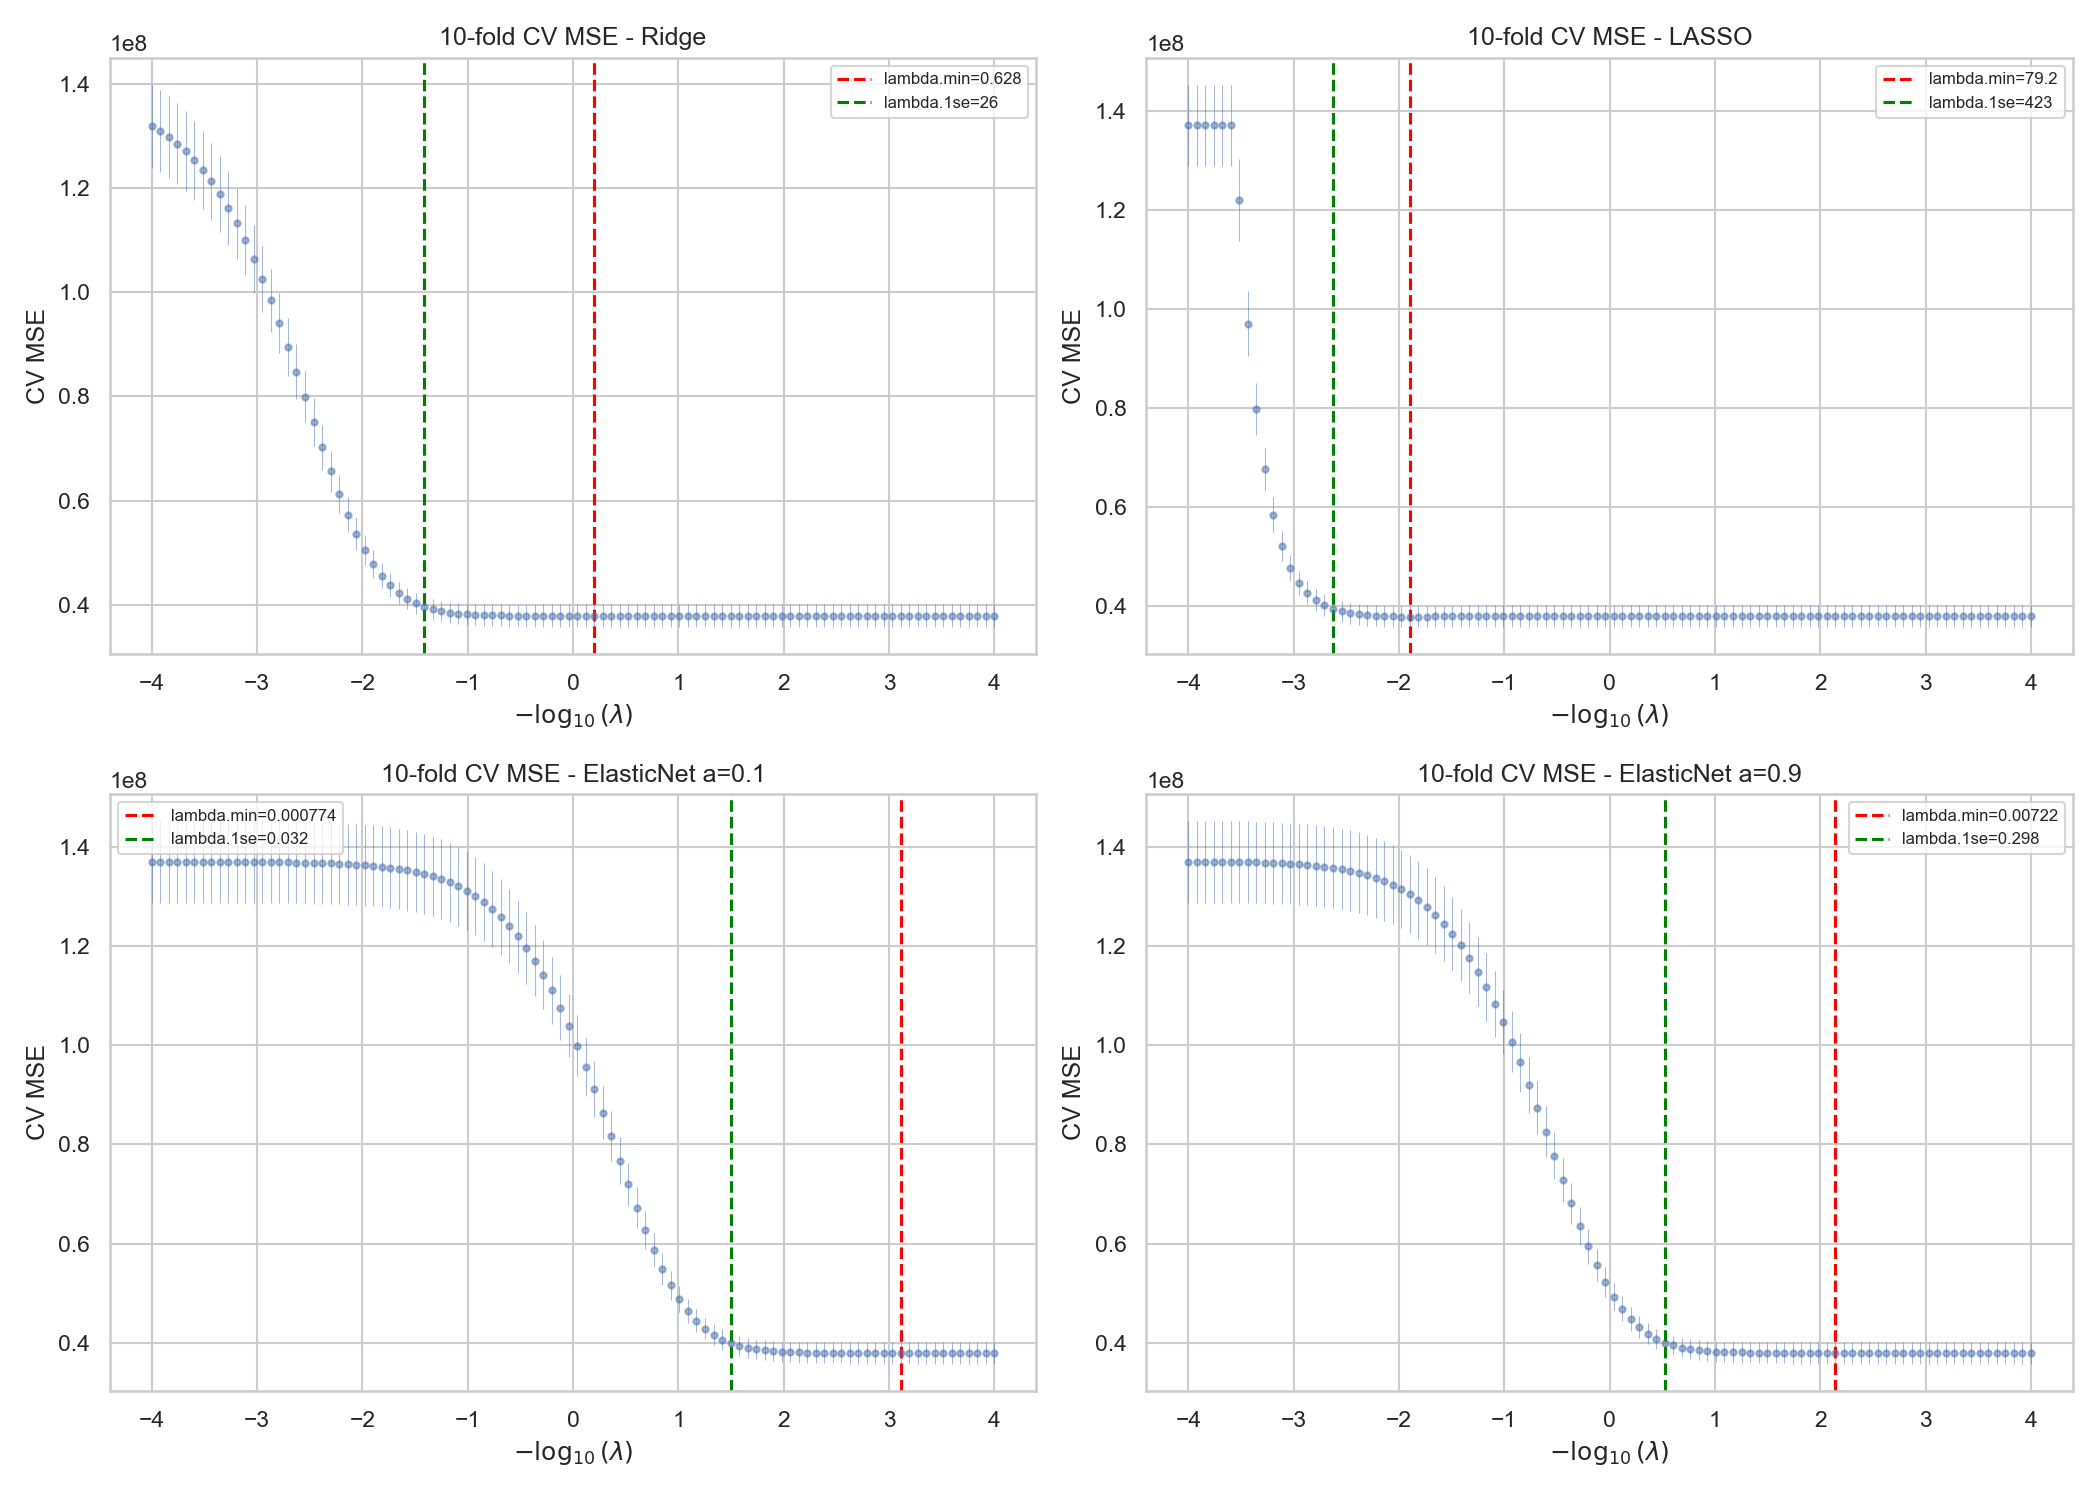
\includegraphics[width=\textwidth]{output/12_cv_mse_vs_loglambda.png}
\caption{10-fold CV MSE in funzione di $-\log_{10}(\lambda)$, con
$\lambda_{min}$ evidenziato (linea rossa).}
\label{fig:cvmse}
\end{figure}

\subsection{Confronto dei modelli}
La Tabella~\ref{tab:regolarizzazione} riassume $\lambda_{min}$, MSE di
cross-validation, MSE e $R^2$ sul test set, e numero di regressori non
nulli per ciascun modello, confrontati con la baseline OLS (senza
regolarizzazione) sullo stesso split.

\begin{table}[H]
\centering
\caption{Confronto dei modelli di regolarizzazione (test set, $n=268$)}
\label{tab:regolarizzazione}
\begin{tabular}{lrrrrr}
\toprule
Modello & $\lambda_{min}$ & Test MSE & Test RMSE & Test $R^2$ & Regr.\ non nulli \\
\midrule
Ridge              & 0.628  & $35.59\times10^6$ & 5\,966 & 0.8063 & 8/8 \\
LASSO              & 79.25  & $36.73\times10^6$ & 6\,060 & 0.8001 & \textbf{4/8} \\
Elastic Net ($\alpha=0.1$) & 0.0008 & $35.62\times10^6$ & 5\,968 & 0.8062 & 8/8 \\
Elastic Net ($\alpha=0.9$) & 0.0072 & $35.62\times10^6$ & 5\,968 & 0.8062 & 8/8 \\
OLS (no reg.)      & 0      & $35.48\times10^6$ & 5\,956 & 0.8069 & 8/8 \\
\bottomrule
\end{tabular}
\end{table}

\begin{figure}[H]
\centering
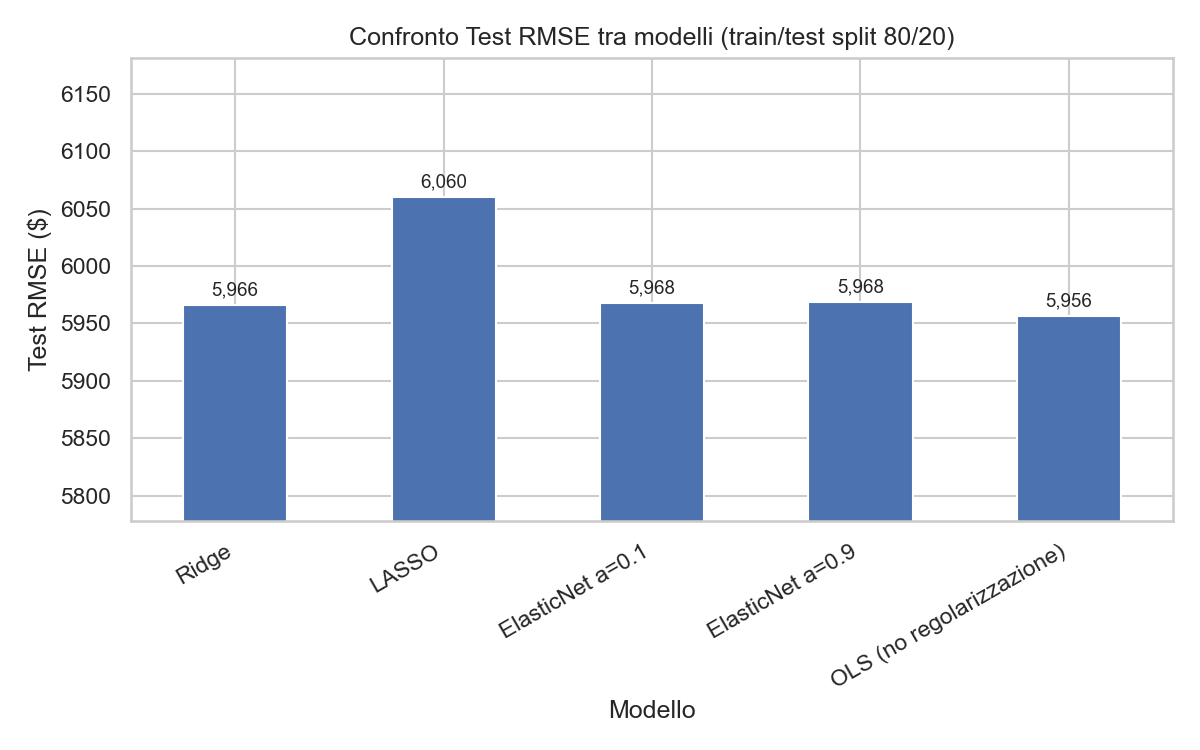
\includegraphics[width=0.75\textwidth]{output/13_test_rmse_comparison.png}
\caption{Confronto del Test RMSE tra i modelli.}
\label{fig:rmse_comparison}
\end{figure}

\textbf{Selezione delle variabili:} LASSO azzera esattamente
\texttt{sex\_male}, \texttt{region\_northwest},\\ \texttt{region\_southeast},
\texttt{region\_southwest}: le \emph{stesse identiche} variabili escluse
dalla Best Subset Selection nello Step~2 (Sezione~3.4). Questa convergenza
tra un criterio classico e uno di
regolarizzazione automatica costituisce una forte
conferma incrociata della robustezza del modello a 4 regressori.

\textbf{Confronto degli MSE:} l'OLS non regolarizzato
ottiene il Test RMSE più basso, per un margine contenuto. Ciò è coerente con la
diagnosi di multicollinearità della Sez.~3.6: la regolarizzazione offre
il massimo vantaggio quando vi è overfitting da collinearità o alta
dimensionalità ($p$ grande rispetto a $n$); qui invece $n=1069\gg p=8$ e i
regressori sono quasi ortogonali (VIF$\approx1$), per cui Ridge ed Elastic
Net convergono a $\lambda_{min}$ vicino a zero (confermato dal fatto che i
$\lambda_{min}$ di Elastic Net si assestano su valori $\ll1$, non sul
bordo della griglia). Il costo del LASSO (RMSE leggermente più alto)
riflette il classico \emph{trade-off} bias-varianza: la penalità L1
introduce una piccola distorsione sui coefficienti sopravvissuti
(es.\ \texttt{bmi}: $1927\to1772$) in cambio di sparsità e
interpretabilità, non di un guadagno predittivo in questo specifico
dataset.

% =======================================================================
\section{Conclusioni}
% =======================================================================

L'analisi ha permesso di individuare  i regressori che influiscono la spesa sanitaria nel dataset \emph{Medical Cost Personal Datasets}:

\begin{enumerate}[nosep]
    \item \textbf{Analisi descrittiva}: \texttt{charges} presenta una
    distribuzione fortemente asimmetrica e bimodale, generata
    principalmente dalla variabile fumatore/non fumatore.
    \item \textbf{Modello inferenziale}: il modello finale
    $\ln(\texttt{charges}) = \beta_0+\beta_1\texttt{age}+\beta_2\texttt{bmi}+\beta_3\texttt{children}+\beta_4\texttt{smoker\_yes}$,
    in forma \textbf{log-lin} (scelta poiché \texttt{charges} è
    strettamente positiva, mentre il modello lin-lin può generare
    previsioni negative, come mostrato in Sezione 3.3), selezionato
    tramite BIC, spiega il 76.2\% della varianza di $\ln(\texttt{charges})$
    ($R^2_{adj}=0.761$) con tutti i coefficienti altamente significativi e
    nessuna multicollinearità rilevante (VIF$\approx1$, $k=291.6$). In
    termini di semi-elasticità, essere fumatori è associato a un aumento
    atteso della spesa del $+367.7\%$, dominando nettamente gli effetti di
    \texttt{age} ($+3.5\%$/anno), \texttt{bmi} ($+1.1\%$/punto) e
    \texttt{children} ($+10.6\%$/figlio). Le variabili \texttt{sex} e
    \texttt{region} non risultano determinanti significativi della spesa
    nella specificazione a 4 regressori.
    \item \textbf{Eteroschedasticità}: confermata formalmente anche nel
    modello log-lin (Breusch-Pagan e White, $p<0.001$). L'inserimento del
    termine di interazione \texttt{smoker\_yes}$\times$\texttt{bmi}
    migliora significativamente il fit ($R^2$ da 0.762 a 0.777, $t=9.37$
    sul coefficiente di interazione, $p<0.001$) ma riduce le statistiche
    LM di soli tra il 5.7\% e il 7.9\%, che restano altamente significative: a
    differenza della specificazione in livelli, in scala log-lin
    l'eteroschedasticità non viene risolta, poiché la trasformazione
    logaritmica ha già assorbito gran parte della relazione
    media-varianza. In termini di semi-elasticità, l'effetto di
    \texttt{bmi} è pressoché nullo per i non fumatori ($+0.09\%$/punto,
    $p=0.695$) e marcato per i fumatori ($+4.61\%$/punto, $p<0.001$),
    spiegando il pattern osservato nell'analisi esplorativa. Data la
    persistenza dell'eteroschedasticità, l'uso di errori standard robusti
    resta consigliabile.
    \item \textbf{Modelli predittivi}: Ridge, LASSO ed Elastic Net non
    migliorano la capacità predittiva rispetto all'OLS (Test RMSE
    compreso tra $\approx\$5\,956$ e $\$6\,060$ in tutti i casi), coerentemente con
    l'assenza di collinearità e la bassa dimensionalità del problema
    ($n\gg p$). Il LASSO conferma però in modo del tutto indipendente,
    tramite selezione automatica via penalità L1, la stessa riduzione a 4
    variabili individuata dalla Best Subset Selection: una validazione
    incrociata robusta della specificazione finale.
\end{enumerate}

\end{document}
